\documentclass[border=12pt]{standalone}
\def\pgfsysdriver{pgfsys-dvisvgm.def}
\usepackage[dvisvgm]{xcolor}
\usepackage{xeCJK}
\setCJKmainfont{HaranoAjiGothic-Regular.otf}[BoldFont=HaranoAjiGothic-Bold.otf]
\setCJKsansfont{HaranoAjiGothic-Regular.otf}[BoldFont=HaranoAjiGothic-Bold.otf]
\usepackage{amsmath,amssymb,tikz,lmodern}
\usetikzlibrary{arrows.meta,positioning,calc,fit,backgrounds}
\renewcommand{\familydefault}{\sfdefault}
\definecolor{ink}{HTML}{25322F}
\definecolor{green}{HTML}{246657}
\definecolor{tint}{HTML}{EEF4F0}
\definecolor{soft}{HTML}{C6D2CC}
\definecolor{muted}{HTML}{52615B}
\newif\ifJapanese
\newcommand{\Tx}[2]{\ifJapanese #1\else #2\fi}
\newcommand{\Eff}{\overline{\operatorname{Eff}}}
\newcommand{\heading}[3]{{\color{green}\bfseries #1\quad\Tx{#2}{#3}}\\[5pt]}
% A white rectangle makes the complete citation label clickable, including spaces.
\newcommand{\refurl}[2]{\special{dvisvgm:raw <a xlink:href="#1" target="_blank" rel="noopener noreferrer">}{\setlength{\fboxsep}{0pt}\colorbox{white}{\color{green}\underline{\strut #2}}}\special{dvisvgm:raw </a>}}
\tikzset{
 card/.style={draw=soft,fill=white,rounded corners=2pt,align=left,text=ink,font=\fontsize{10.5}{14}\selectfont,inner xsep=12pt,inner ysep=10pt,text width=14.4cm},
 half/.style={card,text width=6.45cm,minimum height=2.05cm},
 result/.style={card,draw=green,fill=tint,line width=.9pt},
 reason/.style={align=left,text=muted,font=\fontsize{9}{12}\selectfont,inner sep=0pt,text width=12.7cm},
 branchreason/.style={reason,text width=5.95cm},
 edge/.style={-{Stealth[length=2.4mm]},draw=green,line width=1pt},
 wire/.style={draw=green,line width=1pt},
}
% Keep the arrow in a dedicated left gutter; explanations never cover it.
\newcommand{\flow}[3]{
 \coordinate (#2-from) at ($(#1.south)+(-6.9,0)$);
 \coordinate (#2-to) at ($(#2.north)+(-6.9,0)$);
 \draw[edge] (#2-from)--(#2-to);
 \node[reason,anchor=west] (#2-reason) at ($(#2-from)!.5!(#2-to)+(.55,0)$) {#3};
}

\newcommand{\Cite}[2]{\refurl{#1}{#2}}

\Japanesetrue
\begin{document}
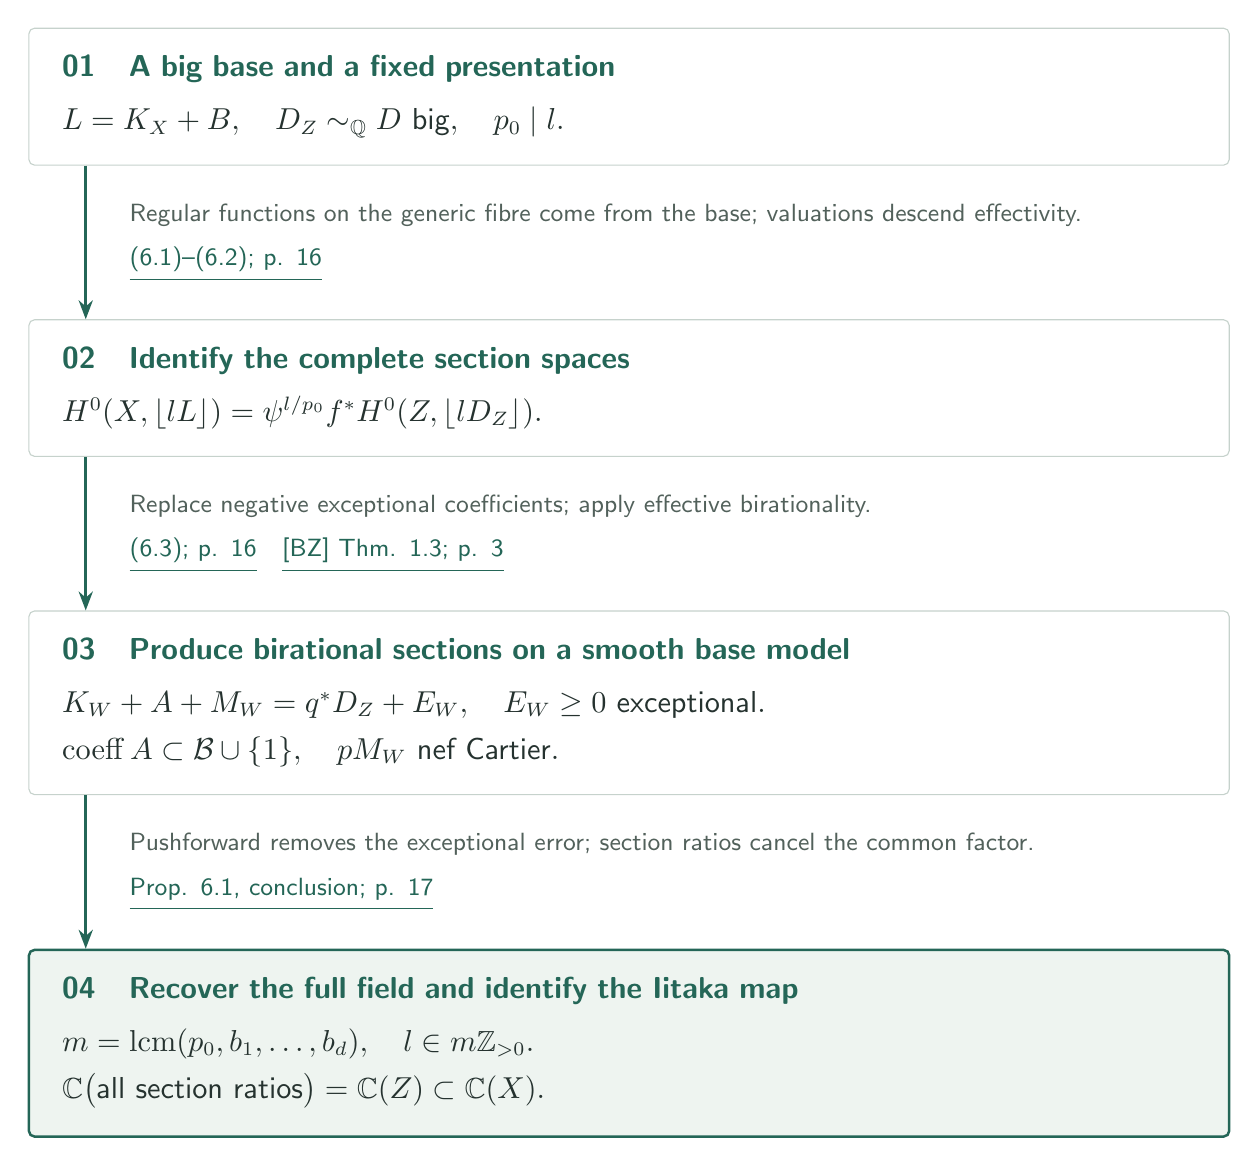
\begin{tikzpicture}
\node[card] (n0) {\heading{01}{bigな底と固定した表示}{A big base and a fixed presentation}$L=K_X+B,\quad D_Z\sim_{\mathbb Q}D\text{ big},\quad p_0\mid l.$};
\node[card,below=1.95cm of n0] (n1) {\heading{02}{完全切断空間を一致させる}{Identify the complete section spaces}$H^0(X,\lfloor lL\rfloor)=\psi^{l/p_0}f^*H^0(Z,\lfloor lD_Z\rfloor).$};
\flow{n0}{n1}{\Tx{一般ファイバー上の正則関数は底の関数。付値でeffectivityを降下。}{Regular functions on the generic fibre come from the base; valuations descend effectivity.}\\[4pt]\Cite{https://github.com/openai/math/blob/adc7f1241b42e322a6451854ab7e4b4c146bf78a/preprints/Relative-denominators-and-effective-systems-for-log-Calabi-Yau-fibrations-September-27-2026/paper.pdf}{(6.1)--(6.2); p. 16}}
\node[card,below=1.95cm of n1] (n2) {\heading{03}{底の滑らかなモデルで双有理切断を作る}{Produce birational sections on a smooth base model}$K_W+A+M_W=q^*D_Z+E_W,\quad E_W\ge0\text{ exceptional}.$\\[3pt] $\operatorname{coeff}A\subset\mathcal B\cup\{1\},\quad pM_W\text{ nef Cartier}.$};
\flow{n1}{n2}{\Tx{負の例外係数を被約例外境界で置換し、有効双有理性を適用。}{Replace negative exceptional coefficients; apply effective birationality.}\\[4pt]\Cite{https://github.com/openai/math/blob/adc7f1241b42e322a6451854ab7e4b4c146bf78a/preprints/Relative-denominators-and-effective-systems-for-log-Calabi-Yau-fibrations-September-27-2026/paper.pdf}{(6.3); p. 16}\quad \Cite{https://arxiv.org/pdf/1410.0938}{[BZ] Thm. 1.3; p. 3}}
\node[result,below=1.95cm of n2] (n3) {\heading{04}{全関数体を得て飯高写像を特定}{Recover the full field and identify the Iitaka map}$m=\operatorname{lcm}(p_0,b_1,\ldots,b_d),\quad l\in m\mathbb Z_{>0}.$\\[3pt] $\mathbb C\bigl(\Tx{\text{全切断比}}{\text{all section ratios}}\bigr)=\mathbb C(Z)\subset\mathbb C(X).$};
\flow{n2}{n3}{\Tx{例外誤差はpushforwardで消え、共通因子は切断比で消える。}{Pushforward removes the exceptional error; section ratios cancel the common factor.}\\[4pt]\Cite{https://github.com/openai/math/blob/adc7f1241b42e322a6451854ab7e4b4c146bf78a/preprints/Relative-denominators-and-effective-systems-for-log-Calabi-Yau-fibrations-September-27-2026/paper.pdf}{Prop. 6.1, conclusion; p. 17}}
\end{tikzpicture}

\end{document}
